% !TEX root = ../Thesis.tex
% !TEX output_directory
\documentclass[11pt,a4paper,english,greek,twoside]{../Thesis}
\begin{document}
\chapter{Ηλεκτροεγκεφαλογραφία}
\section{Βιοηλεκτρικά Σήματα και Ηλεκτροεγκεφαλογράφημα}
%Στο εισαγωγικό κεφάλαιο εστιάσαμε στην σημασία της μελέτης του εγκεφάλου και των σημάτων που μπορούμε να εξάγουμε από αυτόν.
Τα βιοηλεκτρικά σήματα είναι το αποτέλεσμα των ηλεκτροχημικών μεταβολών που λαμβάνουν χώρα εντός και μεταξύ των κυττάρων των νεύρων καθώς και των μυών. Πιο συγκεκριμένα, εάν ένα τέτοιο κύτταρο δεχθεί ερέθισμα ισχυρότερο από ένα κατώφλι συνήθως μεταξύ  -55mV και -50mV, τότε θα παράγει ένα δυναμικό δράσης το οποίο θα μεταδοθεί και θα διεγείρει γειτονικά κύτταρα. Αυτή η ομαδική δραστηριότητα των κυττάρων παράγει ηλεκτρικά πεδία ικανά να ανιχνευτούν με την βοήθεια ηλεκτροδίων τα οποία τοποθετούνται στην επιφάνεια του αντίστοιχου οργάνου, είτε στην δερματική επιφάνεια πάνω αυτό το όργανο. Όταν το ζωτικό αυτό όργανο είναι ο εγκέφαλος τότε το βιοηλεκτρικό σήμα ονομάζεται Ηλεκτροεγκεφαλογράφημα (ΗΕΓ – EEG) και η πρώτη καταγραφή ΗΕΓ, έγινε το 1924 από τον Γερμανό ψυχίατρο Hans Berger. 

Η Ηλεκτροεγκεφαλογραφία, είναι η πρώτη μέθοδος που χρησιμοποιήθηκε για την απεικόνιση της εγκεφαλικής δραστηριότητας, πριν την εμφάνιση μεθόδων όπως η μαγνητική τομογραφία (MRI) και τομογραφία εκπομπής ποζιτρονίων (PET). Παρουσιάζει σημαντικά πλεονεκτήματα όπως το ότι είναι πολύ οικονομικά προσιτή μέθοδος, συγκρινόμενη με τις άλλες που αναφέρθηκαν, και το γεγονός πως έχει πολύ χρονική ανάλυση (temporal resolution), καθώς ενώ οι μεταβολές δυναμικού του εγκεφάλου συμβαίνουν σε πολύ μικρά χρονικά διαστήματα, οι εγκεφαλογράφοι πλέον κάνουν δειγματοληψία του σήματος με συχνότητες έως και $2048Hz$, διατηρώντας σχεδόν όλη την πληροφορία του σήματος. Ωστόσο, όσον αφορά την χωρική ανάλυση (spatial resolution), ισχύει κάτι αντίστοιχο. Τα ηλεκτρικά σήματα από την στιγμή που ξεκινάνε από την πηγή τους, μέχρι να καταλήξουν στα ηλεκτρόδια, διασκορπίζονται κατά την διέλευση τους από το κρανίο. Συνεπώς το σήμα που ανιχνεύεται από ένα ηλεκτρόδιο σε μια συγκεκριμένη περιοχή δεν προέρχεται μόνο από το σημείο του εγκεφάλου που καλύπτει, αλλά και από τα γειτονικά. Αυτό το πρόβλημα αντιμετωπίζεται κάνοντας χρήση περισσότερων ηλεκτροδίων, και χρήσης τεχνικών χωρικού φιλτραρίσματος, για την λύση του αντίστροφου προβλήματος, δηλαδή την εύρεση του πραγματικού ηλεκτρικού σήματος που ξεκίνησε από κάθε περιοχή του εγκεφάλου.
\section{Εγκεφαλογράφος}
Η συσκευή που χρησιμοποιείται για την καταγραφή του εγκεφαλογραφήματος, ονομάζεται εγκεφαλογράφος, και είναι μια πολύπλοκη συσκευή που μπορεί να αναλυθεί σε 5 υποσυστήματα.

\subsection{Ηλεκτρόδια}
Tα ηλεκτρόδια στην πραγματικότητα, είναι μετατροπείς, οι οποίοι ανιχνεύουν την κατανομή των ιόντων στην επιφάνεια των ιστών που καλύπτουν, μετατρέποντας το ιοντικό ρεύμα σε ρεύμα ηλεκτρόνιων. Τα ηλεκτρόδια χωρίζονται σε δύο βασικές κατηγορίες, τα 'υγρά' (wet) και τα 'στεγνά' (dry) και καθένα από αυτά μπορεί να είναι είτε μιας χρήσης, είτε επαναχρησιμοποιούμενο. 
\begin{itemize}
    \item{Υγρά (Wet) Ηλεκτρόδια}
    \par Σε αυτόν τον τύπο, χρησιμοποιείται αγώγιμο υγρό μεταξύ του δέρματος και του ηλεκτροδίου προκειμένου να επιτευχθεί αντίσταση επαφής περίπου $5kΩ$ \cite{}, έτσι ώστε να εξασφαλιστεί καλή ποιότητα σήματος ΗΕΓ με υψηλό λόγο σήματος προς θόρυβο (SNR). Ο συχνότερος τύπος ‘υγρών’ ηλεκτροδίων είναι τα αργύρου-χλωριούχου αργύρου (Ag – AgCL), τα οποία αποτελούνται απο ένα δισκίο, από καθαρό άργυρο $99.9\% $, επικαλυμένα από ένα λεπτό στρώμα χλωριούχου αργύρου. Είναι ευρέως χρησιμοποιούμενα λόγω του χαμηλού κόστους τους, της ευκολίας στην χρήση τους, καθώς και το ότι δεν είναι τοξικά. σε μορφή δισκίων η κυπέλλων \textcolor{red}{(βαλε εικονα)}.  
    \par Ένα άλλο είδος υγρών ηλεκτροδίων, χρησιμοποιούνται στον εγκεφαλογράφο Epoc που κατασκευάζεται από την εταιρεία Emotiv, και αποτελούνται από ένα χάλκινο ηλεκτρόδιο, επικαλυμμένο από μια λεπτή στρώση χρυσού. Η επαφή με το δέρμα γίνεται μέσω ενός κυλινδρικού σφουγγαριού (felt pad), το οποίο διαποτίζετε σε αλατούχο διάλυμα (saline) για την ελάττωση της αντίστασης επαφής.
    \par Παρότι η επίδοση των υγρών ηλεκτροδίων είναι πολύ ικανοποιητική, και χρησιμοποιείται ως σημείο αναφοράς για τις νέες τεχνολογίες ηλεκτροδίων που εμφανίζονται, μια σειρά απο μειονεκτήματα, εμποδίζει την χρήση τους σε περιβάλλοντα εκτός εργαστηρίου. Το πρώτο και βασικότερο είναι η δυσκολία που έχουν στην εφαρμογή τους και η άβολη αίσθηση που έχουν κατά την χρήση τους λόγω του υγρού στοιχείου. Συνήθως, απαιτείται ειδικός καθαρισμός  του σημείου επαφής πριν την χρήση, για την επίτευξη καλύτερου σήματος, αλλά και μετά το πέρας της διαδικασίας, για να καθαριστεί το δέρμα από  τα υπολείμματα του αγώγιμου υγρού. Επιπλέον, η επίτευξη της επιθυμητής αντίστασης που αναφέρθηκε προηγουμένως, μπορεί να καθυστερήσει σημαντικά. Τέλος, λόγω της πτητικότητας του αγώγιμου υγρού, υπάρχει ένα μικρό περιθώριο λίγων ωρών, πριν να ξαναχρειαστεί να το ανανεώσουμε. Όλοι αυτοί οι λόγοι είναι που εμποδίζουν την ευρεία χρήση των εγκεφαλογράφων εκτός των εργαστηρίων, σε πραγματικές καθημερινές εφαρμογές.
    
    \item{Στεγνά (Dry) Ηλεκτρόδια}
    \par Τα προηγούμενα μειονεκτήματα έρχεται να τα καλύψει μια νέα τεχνολογία ηλεκτροδίων που δεν χρησιμοποιούν κάποιο αγώγιμο υγρό, αλλά εκμεταλλεύονται τις εξελίξεις στον τομέα τεχνολογίας υλικών και των μικρο-συστημάτων (MEMS). Τα ηλεκτρόδια αυτά έχουν 

    των τελεστικών ενισχυτών οργανολογίας (instrumental amplifiers) και τις


\end{itemize}
\subsection{Ενισχυτής}

\subsection{Μονάδα Επεξεργασίας}

\subsection{Απεικόνιση Σημάτων}

\section{Σύστημα 10-20}
Το σύστημα 10-20 χρησιμοποιείται διεθνώς για να περιγράψει και να ορίσει την θέση των ηλεκτροδίων στο κεφάλι. Η χρήση ενός τέτοιου συστήματος είναι απαραίτητη, προκειμένου να υπάρχει ένα κοινό σημείο αναφοράς μεταξύ των ερευνητών για την αναπαραγωγή και σύγκριση των διαφόρων μεθοδολογιών στην εγκεφαλογραφία.
Οι αριθμοί $'10'$ και $'20'$ είναι ποσοστά και συμβολίζουν το $10\% $ και $20\% $  της απόστασης μεταξύ των δύο αυτιών, τα οποία με την σειρά τους ορίζουν την απόσταση από ένα αυτί προς το πλησιέστερο σε αυτό ηλεκτρόδιο και την απόσταση μεταξύ δύο γειτονικών ηλεκτροδίων αντίστοιχα.

\begin{figure}[h]
  \centering
  \noindent\makebox[\textwidth]{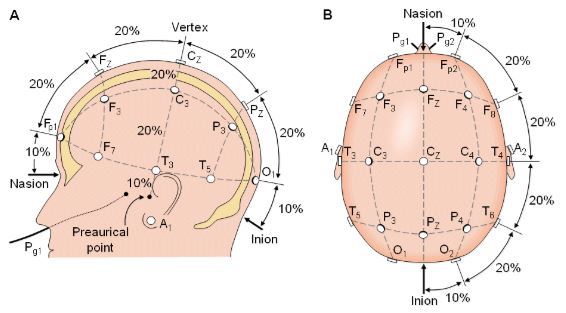
\includegraphics[scale=1]{{ImagesSSVEP/10_20}.jpg}}
  \captionsetup{singlelinecheck = false, justification=justified} % used for left alignment
  \caption{Τοποθεσίες ηλεκτροδίων με βάση το σύστημα 10-20.\\ Εικόνα από \cite{Malmivuo2012Bioelectromagnetism:Fields}. }
  \label{fig:10_20}
\end{figure}

Ανάλογα με την εγκεφαλική περιοχή που καλύπτουν τα ηλεκτρόδια, παίρνουν και το όνομά τους που αποτελείται από ένα γράμμα (η συνδυασμό γραμμάτων) και έναν ζυγό αριθμό για το δεξί ημισφαίριο και περιττό για το αριστερό ημισφαίριο. Η βασική διάταξη που αποτελείται από 19 ηλεκτρόδια, είναι η εξής :

\begin{itemize}
    \item Προμετωπιαίος φλοιός (Pre-Frontal cortex) : Fp1, Fp2
    \item Μετωπιαίος λοβός (Frontal lobe) : F3, F4, F7, F8, Fz
    \item Κροταφικός λοβός (Temporal lobe) : T3, T4, T5, T6
    \item Βρεγματικός λοβός (Parietal lobe) : P3, P4, Pz
    \item Ινιακός λοβός (Occipital lobe) : O1, O2
    \item Κεντρική περιοχή (Central) : C3, C4, Cz
\end{itemize}
\par Ο δείκτης z, προσδιορίζει τα ηλεκτρόδια τα οποία βρίσκονται πάνω στην διαχωριστική γραμμή μεταξύ των δύο ημισφαιρίων.
Το παραπάνω σύστημα μπορεί να επεκταθεί έτσι ώστε να καλύψει καταστάσεις στις οποίες απαιτείται μεγαλύτερος αριθμός ηλεκτροδίων, ορίζοντας νέες εγκεφαλικές περιοχές μεταξύ αυτών που αναφέρθηκαν, ή και διαφορετικές σχετικές αποστάσεις μεταξύ των ηλεκτροδίων.
\begin{figure}[h]
  \centering
  \noindent\makebox[\textwidth]{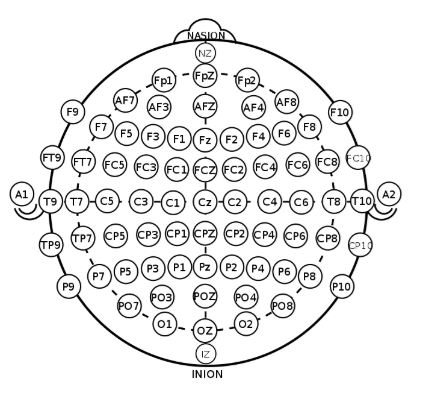
\includegraphics[scale=1]{{ImagesSSVEP/10_20_ext}.jpg}}
  \captionsetup{singlelinecheck = false, justification=justified} % used for left alignment
  \caption{Επέκταση συστήματος 10-20 .\\ Εικόνα από \cite{Malmivuo2012Bioelectromagnetism:Fields}. }
  \label{fig:10_20_ext}
\end{figure}

\cite{Meng2011ABCI} 
\end{document}
